
% This LaTeX was auto-generated from MATLAB code.
% To make changes, update the MATLAB code and republish this document.

\documentclass{article}
\usepackage{graphicx}
\usepackage{color}

\sloppy
\definecolor{lightgray}{gray}{0.5}
\setlength{\parindent}{0pt}

\begin{document}

    
    
\section*{TIP7200 - Processamento Digital de Sinais - HW 2}

\begin{par}
Author: Lucas Abdalah
\end{par} \vspace{1em}
\begin{par}
script.m
\end{par} \vspace{1em}
\begin{par}
2023/04/22 - v1
\end{par} \vspace{1em}

\subsection*{Contents}

\begin{itemize}
\setlength{\itemsep}{-1ex}
   \item Preamble
   \item Problem 1
   \item Problem 2
   \item Problem 3
   \item Problem 4
   \item Problem 5
   \item Problem 6
   \item Author Functions
\end{itemize}


\subsection*{Preamble}

\begin{verbatim}
close all;
clearvars;
% clc;
pause(0.1);
% pause off;

savefigPath = '..\figures\';
color_ = struct('X', 'blue', ...
  'Y', 'cyan', ...
  'Yfilt', 'red', ...
  'Xfilt', 'magenta', ...
  'Ex2', [0.3010 0.7450 0.9330], ...
  'Ex3', [0.6350 0.0780 0.1840]);
\end{verbatim}


\subsection*{Problem 1}

\begin{verbatim}
fileName = 'bipsIN';
fprintf('Problema 1 - %s \n\n', fileName);
[x, Fs] = audioread(['data\', fileName, '.wav']);
% Time and Frequencia Domain Analysis
hw2p1fig1 = plot_signal(x, Fs, 'shifted', fileName, color_.X);
\end{verbatim}

        \color{lightgray} \begin{verbatim}Problema 1 - bipsIN 

\end{verbatim} \color{black}
    
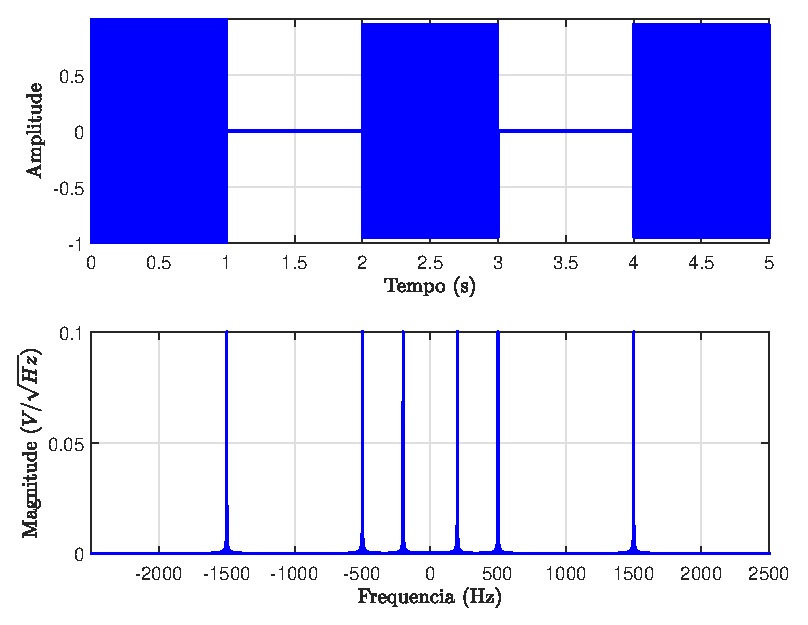
\includegraphics [width=4in]{script_01.eps}


\subsection*{Problem 2}

\begin{verbatim}
fileName = 'bipsOUT';
fprintf('Problema 2 - %s \n\n', fileName)
[y, Fs] = audioread(['data\', fileName, '.wav']);
% Time and Frequencia Domain Analysis
hw2p2fig1 = plot_signal(y, Fs, 'shifted', fileName, color_.Y);

% Low Pass Filter (LPF) - Butterworth
Fcutoff = 250;
Fc_norm = Fcutoff/(Fs/2);
[b,a] = butter(7, Fc_norm);
yfilt = filter(b,a,x);

% Time and Frequencia Domain Analysis
hw2p2fig2 = plot_signal(yfilt, Fs, 'shifted', 'Filter Output', color_.Yfilt);
hw2p2fig3 = figure('name', 'Resposta ao Impulso e em Frequencia');
subplot(2,1,1);
plot_impz(b,a, 'Resposta ao Impulso', color_.Yfilt)
title('Resposta ao Impulso')
subplot(2,1,2)
plot_pspectrum(yfilt, Fs, 'Resposta em Frequencia', color_.Yfilt)
title('Resposta em Frequencia')
\end{verbatim}

        \color{lightgray} \begin{verbatim}Problema 2 - bipsOUT 

\end{verbatim} \color{black}
    
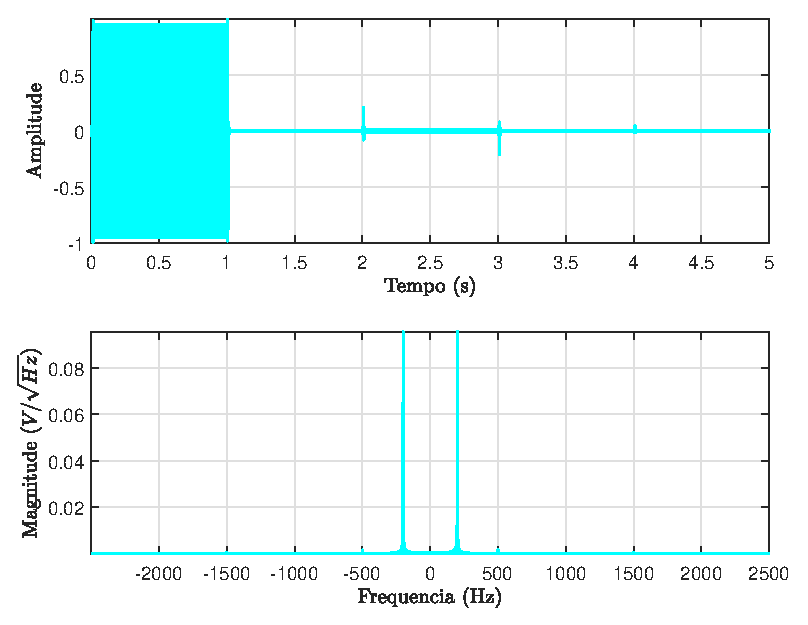
\includegraphics [width=4in]{script_02.eps}

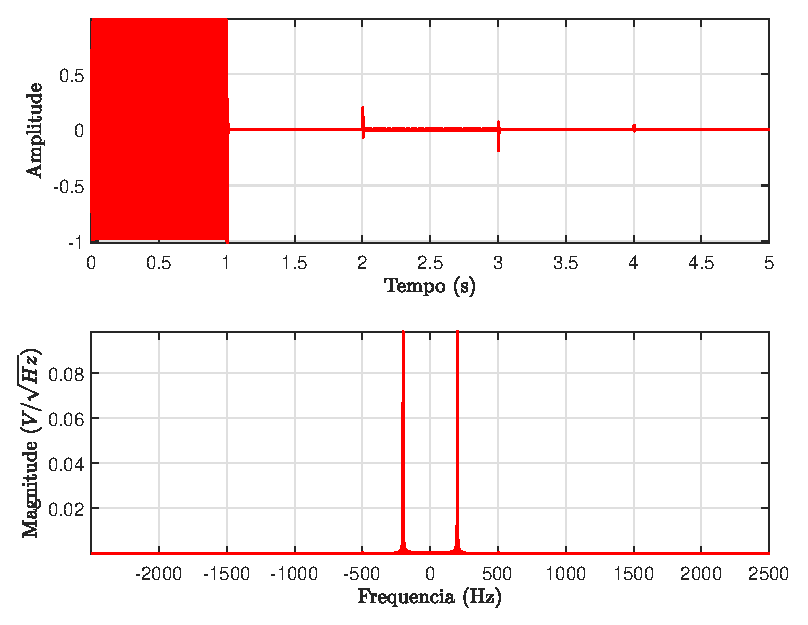
\includegraphics [width=4in]{script_03.eps}

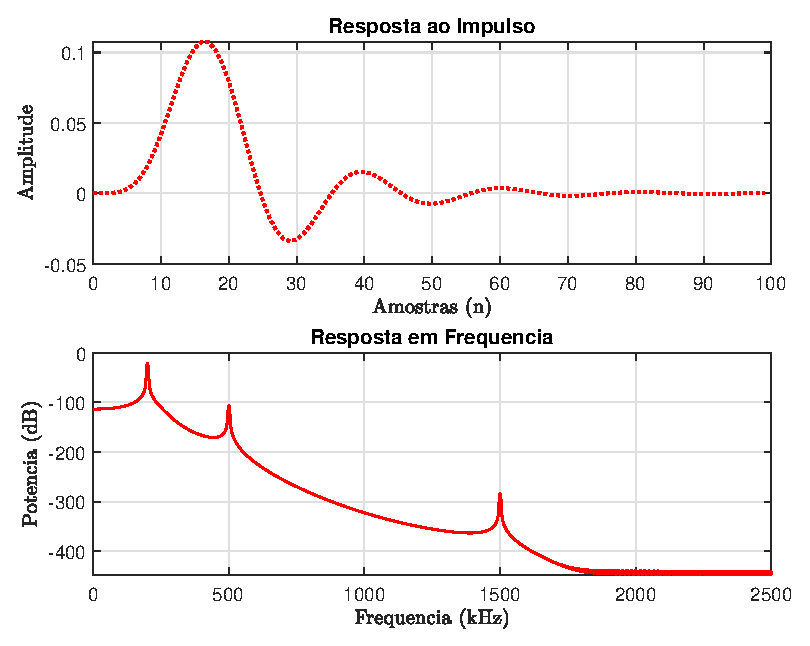
\includegraphics [width=4in]{script_04.eps}


\subsection*{Problem 3}

\begin{par}
Input
\end{par} \vspace{1em}
\begin{verbatim}
fileName = 'bipsIN_mixed';
fprintf('Problema 3 - %s \n\n', fileName)
[x, Fs] = audioread(['data\', fileName, '.wav']);
% Input - Time and Frequencia Domain Analysis
hw2p3fig1 = plot_signal(x, Fs, 'shifted', fileName, color_.X);

% Output - Time and Frequencia Domain Analysis
fileName = 'bipsOUT_mixed';
[y, Fs] = audioread(['data\', fileName, '.wav']);
fprintf('- %s \n\n', fileName)
hw2p3fig2 = plot_signal(y, Fs, 'shifted', fileName, color_.Y);
hw2p3fig3 = figure('name', 'Resposta em Frequencia');
plot_pspectrum(y, Fs, 'Resposta em Frequencia', color_.Y)
pbaspect([2 1 1]);

% Low Pass Filter (LPF) - Butterworth
Fcutoff = 450;
order = 11;
b = fir1(order, Fcutoff/Fs, 'low', kaiser(order+1)); % ,chebwin(35,30))
a = Fcutoff*1e-3;
yfilt = filtfilt(b, a, x);

% Time and Frequencia Domain Analysis
hw2p3fig4 = plot_signal(yfilt, Fs, 'shifted', 'Filter Output', color_.Yfilt);
hw2p3fig5 = figure('name', 'Resposta ao Impulso e em Frequencia');
subplot(2,1,1);
plot_impz(b, a, 'Resposta ao Impulso', color_.Yfilt)
subplot(2,1,2)
plot_pspectrum(yfilt, Fs, 'Resposta em Frequencia', color_.Yfilt)
\end{verbatim}

        \color{lightgray} \begin{verbatim}Problema 3 - bipsIN_mixed 

- bipsOUT_mixed 

\end{verbatim} \color{black}
    
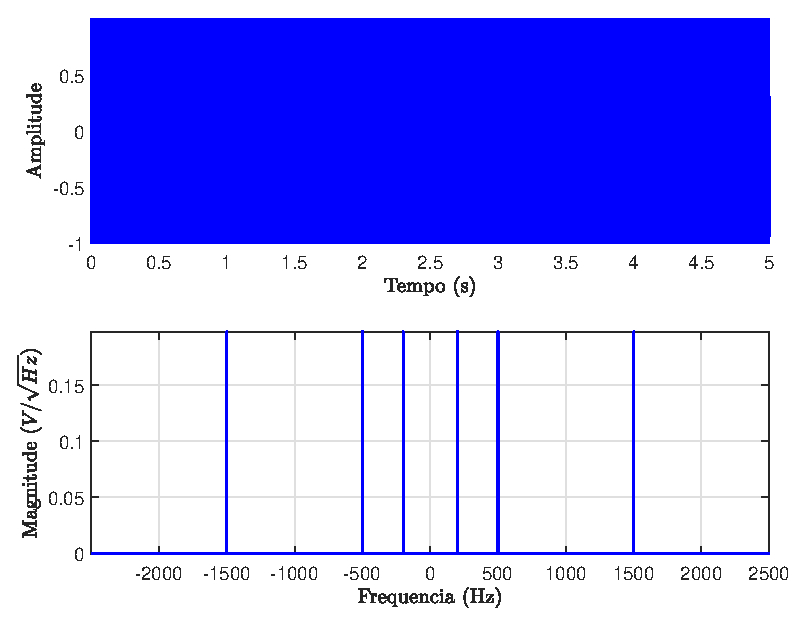
\includegraphics [width=4in]{script_05.eps}

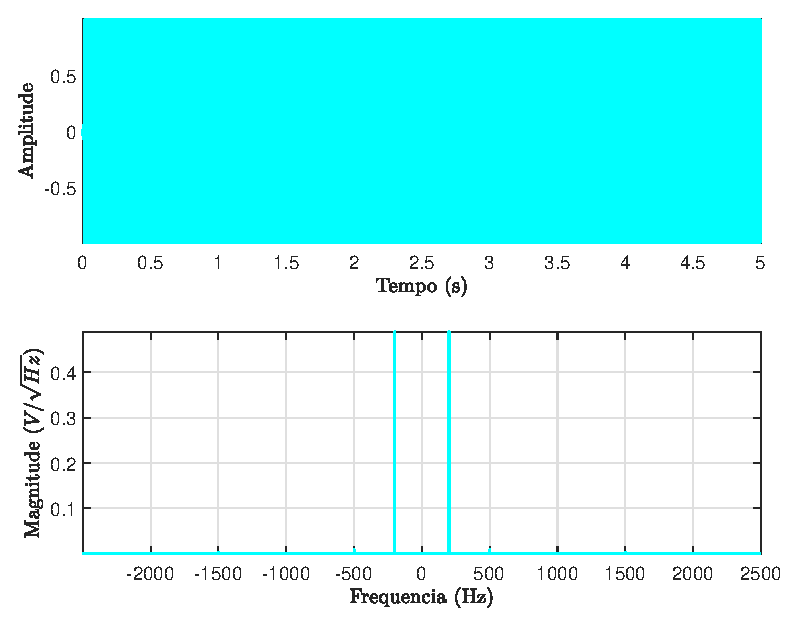
\includegraphics [width=4in]{script_06.eps}

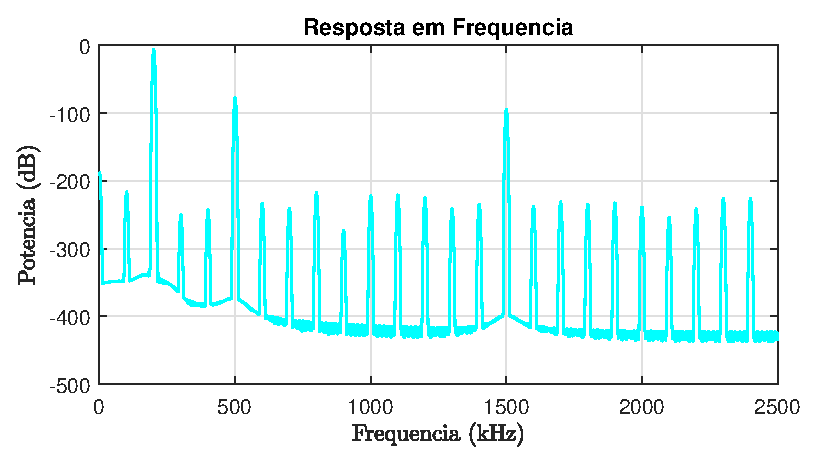
\includegraphics [width=4in]{script_07.eps}

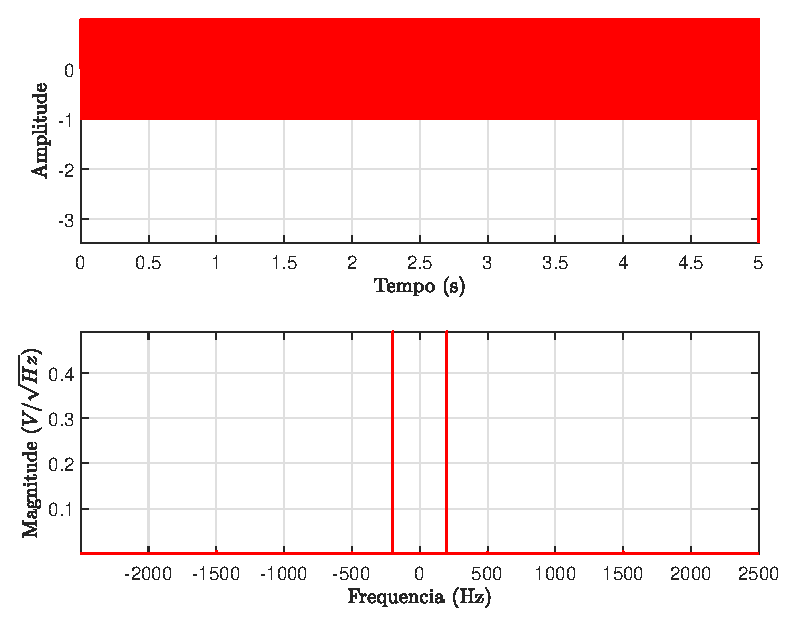
\includegraphics [width=4in]{script_08.eps}

\includegraphics [width=4in]{script_09.eps}


\subsection*{Problem 4}

\begin{par}
Input audio
\end{par} \vspace{1em}
\begin{verbatim}
fileName = 'bomdia';
fprintf('Problema 4 - %s \n\n', fileName);
[x, Fs] = audioread(['data\', fileName, '.wav']);
% Time and Frequencia Domain Analysis
hw2p4fig1 = plot_signal(x, Fs, 'shifted', fileName, color_.X);

% Output audio
fileName = 'bomdia_reverb';
[y, Fs] = audioread(['data\', fileName, '.wav']);
% Time and Frequencia Domain Analysis
hw2p4fig2 = plot_signal(y, Fs, 'shifted', fileName, color_.Y);

% Impulsive response
fileName = 'imp_resp';
reverb = load('data/imp_resp.mat');
hw2p4fig3 = figure('name', 'Resposta ao Impulso');
plot(reverb.h, 'Color', color_.Yfilt, 'LineStyle', ':', 'LineWidth', 1.5);
% title('Resposta ao Impulso')
xlabel('Amostras (n)', 'interpreter', 'Latex');
ylabel('Amplitude', 'interpreter', 'Latex');
pbaspect([2 1 1]);

% Convolve input x and system h
yfilt = conv(x, reverb.h);
hw2p4fig4 = plot_signal(yfilt, Fs, 'shifted', [fileName, ' Convolution'], color_.Yfilt);
\end{verbatim}

        \color{lightgray} \begin{verbatim}Problema 4 - bomdia 

\end{verbatim} \color{black}
    
\includegraphics [width=4in]{script_10.eps}

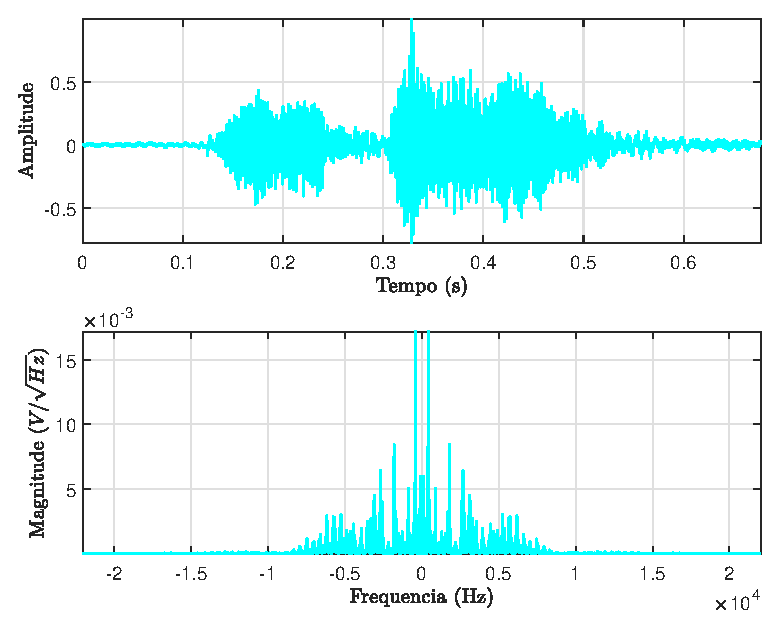
\includegraphics [width=4in]{script_11.eps}

\includegraphics [width=4in]{script_12.eps}

\includegraphics [width=4in]{script_13.eps}


\subsection*{Problem 5}

\begin{par}
Equalizer
\end{par} \vspace{1em}
\begin{verbatim}
fprintf('Problema 5\n\n');
xfilt = retrieve(y, reverb.h);
audiowrite('..\audio\bomdia_restored.wav', xfilt, Fs)
hw2p5fig1 = plot_signal(xfilt, Fs, 'shifted', [fileName, ' Equalized'], color_.Xfilt);

% Error
hw2p5fig2 = figure('name', 'Squared Error ');
sqerror = (x - xfilt).^2;
plot_time(sqerror, Fs, [], color_.Xfilt);
hold on
sqerror_mean = repelem(mean(sqerror), length(sqerror));
plot_time(sqerror_mean, Fs, [], []); % Error
hold off;
legend('$\sum_{n=1}^{N} || a[n] - \hat{a}||^2$', ...
sprintf('$Media = %1.0e$', mean(sqerror)), 'interpreter', ...
  'Latex', 'Location', 'northeast','Orientation', 'Vertical');
axis tight
%}
\end{verbatim}

        \color{lightgray} \begin{verbatim}Problema 5

\end{verbatim} \color{black}
    
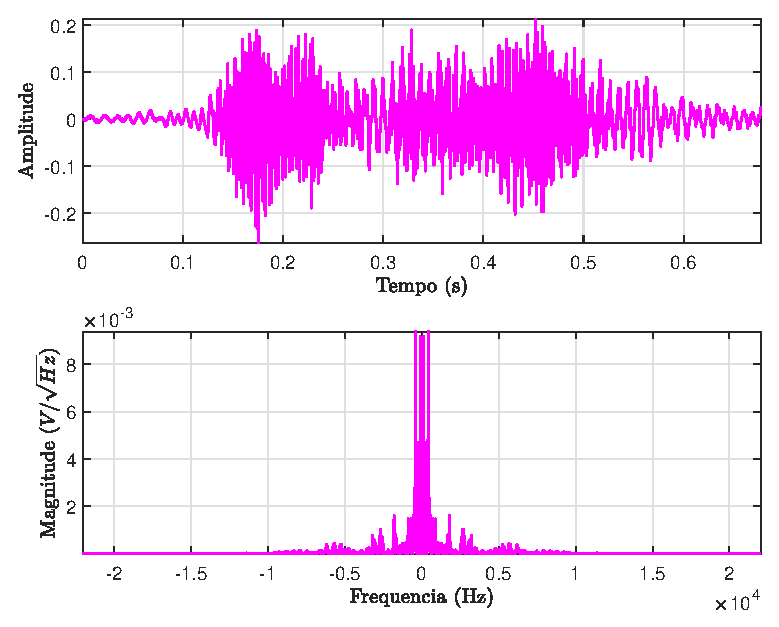
\includegraphics [width=4in]{script_14.eps}

\includegraphics [width=4in]{script_15.eps}


\subsection*{Problem 6}

\begin{par}
Input audio
\end{par} \vspace{1em}
\begin{verbatim}
reverb = load('data/imp_resp.mat');
fileName = 'preamble';
fprintf('Problema 6 - %s \n\n', fileName);
[x, Fs] = audioread(['data\', fileName, '.wav']);
% Time and Frequencia Domain Analysis
hw2p6fig1 = plot_signal(x, Fs, 'shifted', fileName, color_.X);

% Convolve input x and system h, export y
y = conv(x, reverb.h, 'same');
audiowrite('..\audio\preamble_reverb.wav', y, Fs)
hw2p6fig2 = plot_signal(y, Fs, 'shifted', [fileName, ' Convolution'], color_.Y);

% Equalizer
fprintf('Equalizer\n\n');
xfilt = retrieve(y, reverb.h);
audiowrite('..\audio\preamble_restored.wav', xfilt, Fs)
hw2p6fig3 = plot_signal(xfilt, Fs, 'shifted', [fileName, ' Equalized'], color_.Xfilt);

% Error
hw2p6fig4 = figure('name', 'Squared Error ');
sqerror = (x - xfilt).^2;
plot_time(sqerror, Fs, [], color_.Xfilt);
hold on
sqerror_mean = repelem(mean(sqerror), length(sqerror));
plot_time(sqerror_mean, Fs, [], []); % Error
hold off;
legend('$\sum_{n=1}^{N} || a[n] - \hat{a}||^2$', ...
  sprintf('$Media = %1.0e$', mean(sqerror)), 'interpreter', ...
  'Latex', 'Location', 'northwest','Orientation', 'Vertical');
axis tight


% Export figures as eps
%{
saveaseps(hw2p1fig1, 'hw2p1fig1', savefigPath)
saveaseps(hw2p2fig1, 'hw2p2fig1', savefigPath)
saveaseps(hw2p2fig2, 'hw2p2fig2', savefigPath)
saveaseps(hw2p2fig3, 'hw2p2fig3', savefigPath)
saveaseps(hw2p3fig1, 'hw2p3fig1', savefigPath)
saveaseps(hw2p3fig2, 'hw2p3fig2', savefigPath)
saveaseps(hw2p3fig3, 'hw2p3fig3', savefigPath)
saveaseps(hw2p3fig4, 'hw2p3fig4', savefigPath)
saveaseps(hw2p3fig5, 'hw2p3fig5', savefigPath)
saveaseps(hw2p4fig1, 'hw2p4fig1', savefigPath)
saveaseps(hw2p4fig2, 'hw2p4fig2', savefigPath)
saveaseps(hw2p4fig3, 'hw2p4fig3', savefigPath)
saveaseps(hw2p4fig4, 'hw2p4fig4', savefigPath)
saveaseps(hw2p5fig1, 'hw2p5fig1', savefigPath)
saveaseps(hw2p5fig2, 'hw2p5fig2', savefigPath)
saveaseps(hw2p6fig1, 'hw2p6fig1', savefigPath)
saveaseps(hw2p6fig2, 'hw2p6fig2', savefigPath)
saveaseps(hw2p6fig3, 'hw2p6fig3', savefigPath)
saveaseps(hw2p6fig4, 'hw2p6fig4', savefigPath)
%}
\end{verbatim}

        \color{lightgray} \begin{verbatim}Problema 6 - preamble 

Equalizer

\end{verbatim} \color{black}
    
\includegraphics [width=4in]{script_16.eps}

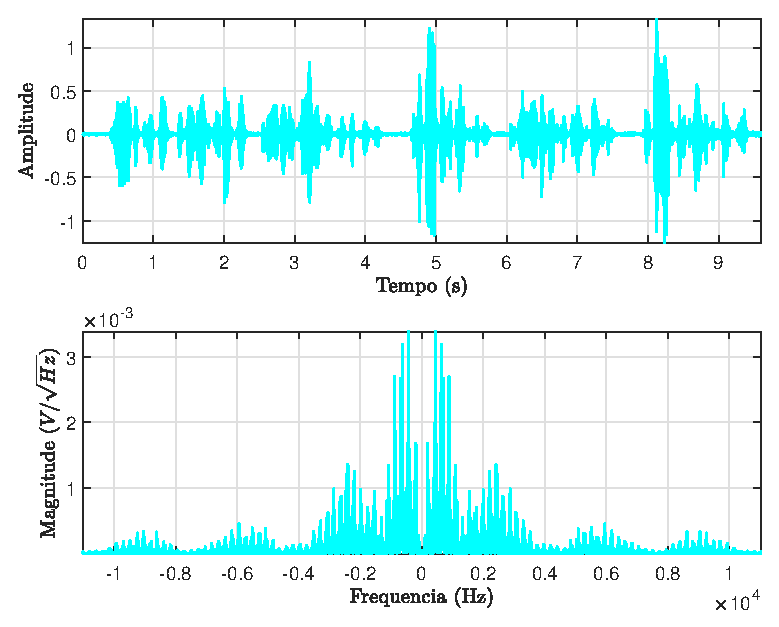
\includegraphics [width=4in]{script_17.eps}


\subsection*{Author Functions}

\begin{verbatim}
function xfilt = retrieve(x, h)
  nPoints = 2e7;
  w = ifft(1./fft(h, nPoints), nPoints);
  xfilt = filter(w, 1, x);
end


function h = plot_signal(x, Fs, approach, figTitle, color)
  h = figure('name', sprintf('Signal Plot: Time and Frequencia Domain - %s', figTitle));
  subplot(2,1,1);
  title('Tempo')
  plot_time(x, Fs, figTitle, color);
  axis tight
  subplot(2,1,2);
  title('Frequencia')
  fft_dsp(x, Fs, approach, figTitle, color);
  axis tight
end


function [t] = plot_time(x, Fs, figTitle, color)
  if isempty(color); color = 'black'; end
  n = length(x);
  t = linspace(0, n/Fs, n);
  % h = figure('name', sprintf('Signal Plot: Time Domain - %s', figTitle));
  plot(t, x, 'Color', color, 'LineStyle', '-', 'LineWidth', 1.0);
  grid on;
  xlabel('Tempo (s)', 'interpreter', 'Latex');
  ylabel('Amplitude', 'interpreter', 'Latex');
  ylim([-1.1 1.1])
end


function [Xf, f] = fft_dsp(x, Fs, approach, figTitle, color)
  if isempty(color); color = 'black'; end

  if nargin < 3 || isempty(approach)
    approach = 'positive';
    figTitle = 'Signal';
  end
  if nargin < 4 || isempty(figTitle)
    figTitle = 'Signal';
  end

  n = length(x);
  xdft = fft(x);

  approachChoice = false; % Fix wrong choices for approach

  while ~approachChoice
    approachChoice = true;

    switch approach

      case 'positive'
          n_positive = fix(n/2)+1;
          f = linspace(0, 1, n_positive)*(Fs/2);  % Positive Frequency
          Xf = abs(xdft(1:length(f)))*2/n;      % Multiply By ‘2’ to scale magnitude since we use half Frequency
          % h = figure('name', sprintf('Positive FFT(x) - %s', figTitle));
          disp(figTitle)
          plot(f, Xf, 'Color', color, 'LineStyle', '-', 'LineWidth', 1.0)
          xlabel('Frequencia (Hz)', 'interpreter', 'Latex')
          ylabel('Magnitude ($V/\sqrt{Hz}$)', 'interpreter', 'Latex')
          xlim([min(f) max(f)])
          ylim([0.9*min(Xf), 1.1*max(Xf)])
          grid on
        case 'shifted'
          xdftShift = fftshift(xdft);
          f = (-n/2+1:n/2)*(Fs/n);  % zero-centered Frequency range
          Xf = abs(xdftShift)/n;  % zero-centered magnitude
          % h = figure('name', sprintf('Reflected FFT(x) - %s', figTitle));
          plot(f,Xf, 'Color', color, 'LineStyle', '-', 'LineWidth', 1.0)
          xlabel('Frequencia (Hz)', 'interpreter', 'Latex')
          ylabel('Magnitude ($V/\sqrt{Hz}$)', 'interpreter', 'Latex')
          xlim([min(f) max(f)])
          ylim([0.9*min(Xf), 1.1*max(Xf)])
          grid on
        case 'freq_norm'
          n_positive = fix(n/2)+1;
          f = linspace(0, 1, n_positive);     % Positive Frequency
          Xf = abs(xdft(1:length(f)))*2/n;  % Multiply By ‘2’ to scale magnitude since we use half Frequency
          % h = figure('name', sprintf('Normalized Frequency FFT(x) - %s', figTitle));
          plot(f, Xf, 'Color', color, 'LineStyle', '-', 'LineWidth', 1.0)
          xlabel('Normalized Frequencia ($\times \pi radians/samples$)', 'interpreter', 'Latex')
          ylabel('Magnitude', 'interpreter', 'Latex')
          xlim([min(f) max(f)])
          grid on
        case 'dB'
          xdft = xdft(1:n/2+1);
          psdx = (1/(Fs*n)) * abs(xdft).^2;
          psdx(2:end-1) = 2*psdx(2:end-1);
          f = 0:Fs/length(x):Fs/2;
          Xf = pow2db(psdx);
          % h = figure('name', sprintf('Positive FFT(x) in dB - %s', figTitle));
          plot(f, Xf, 'Color', color, 'LineStyle', '-', 'LineWidth', 1.0)
          grid on
          xlabel('Frequencia (Hz)', 'interpreter', 'Latex')
          ylabel('Power/Frequencia (dB/Hz)', 'interpreter', 'Latex')
          ylim([-80 10])
        otherwise
          warning("Invalid approach. Replaced by 'positive'")
          approachChoice = false; % Return to switch beginning
          approach = 'positive';
    end
  end

end


function saveaseps(input, saveName, savefigPath)
  saveas(input, sprintf('%s%s', savefigPath, saveName),'epsc')
end


function h = plot_impz(b, a, figTitle, color)
  if isempty(color); color = 'black'; end
    [h_, t] = impz(b, a, 100);
    % h = figure('name', sprintf('Impulse Response Plot: Time Domain - %s', figTitle));
    plot(t, h_, 'Color', color, 'LineStyle', ':', 'LineWidth', 1.5);
    grid on;
    title(figTitle)
    xlabel('Amostras (n)', 'interpreter', 'Latex');
    ylabel('Amplitude', 'interpreter', 'Latex');
end


function h = plot_pspectrum(x, Fs, figTitle, color)
  if isempty(color); color = 'black'; end
  [p,f] = pspectrum(x, Fs);
  % h = figure('name', sprintf('Power spectrum: Frequency Domain - %s', figTitle));
  plot(f, mag2db(p), 'Color', color, 'LineStyle', '-', 'LineWidth', 1.0);
  grid on;
  title(figTitle);
  xlabel('Frequencia (kHz)', 'interpreter', 'Latex');
  ylabel('Potencia (dB)', 'interpreter', 'Latex');
end
\end{verbatim}



\end{document}

